\chapter{Design}
\section{Scope}
\section{Threat model}
\section{Security properties}
\section{Requirements}
\section{Architecture}
\begin{figure}[h]
	\centering
	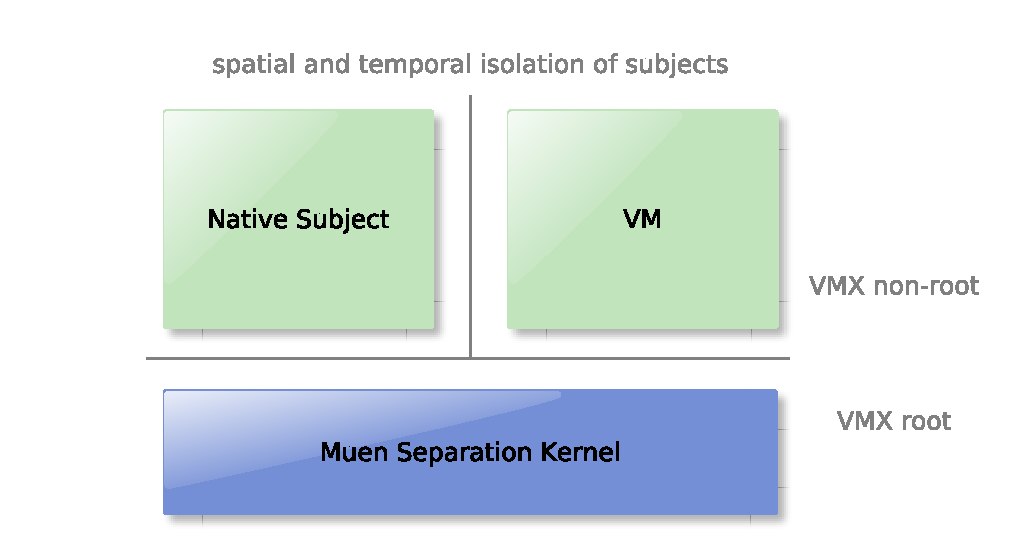
\includegraphics[scale=0.7]{images/architecture-overview}
	\caption{Architecture overview}
	\label{fig:architecture-overview}
\end{figure}

\subsection{Virtualization}
\subsection{Scheduling}

An example scheduling plan is depicted in figure
\ref{fig:example-scheduling-plan}. It illustrated a system with two logical CPUs
that execute various subjects indicated by different colors. Since major frames
are repeated, major frame one and two are identical. All CPUs of the system
wait on a barrier at the beginning of a new major frame. This guarantees that
all logical CPUs of a system are in-sync on major frame changes

CPU 0 is executing the same subject for the whole duration of the major frame.
This could for example be the $\tau$0 subject executing on the bootstrap
processor (BSP). The second CPU is executing two subjects (blue and green) in
alternating order. As can be seen, subject green is granted more CPU cycles than
subject blue.

\begin{figure}[ht]
	\begin{ganttchart}[
		vgrid={*9{dotted},*1{dashed},*9{dotted}},
		hgrid,
		y unit title=0.75cm,
		title label anchor/.style={below=-1.5ex}]{20}
		\gantttitle{Major frame 1}{10}
		\gantttitle{Major frame 2}{10} \\
		\ganttbar[bar/.append style={fill=Apricot}]{CPU 0}{1}{10}
		\ganttbar[bar/.append style={fill=Apricot}]{}{11}{20} \\
		\ganttbar[bar/.append style={fill=CornflowerBlue}]{CPU 1}{1}{2}
		\ganttbar[bar/.append style={fill=YellowGreen}]{}{3}{6}
		\ganttbar[bar/.append style={fill=CornflowerBlue}]{}{7}{8}
		\ganttbar[bar/.append style={fill=YellowGreen}]{}{9}{10}
		\ganttbar[bar/.append style={fill=CornflowerBlue}]{}{11}{12}
		\ganttbar[bar/.append style={fill=YellowGreen}]{}{13}{16}
		\ganttbar[bar/.append style={fill=CornflowerBlue}]{}{17}{18}
		\ganttbar[bar/.append style={fill=YellowGreen}]{}{19}{20}
	\end{ganttchart}
	\caption{Example scheduling plan}
	\label{fig:example-scheduling-plan}
\end{figure}

Figure \ref{fig:example-scheduling-plan-of-a-cpu} illustrates the scheduling
plan for a specific CPU. The major frame consists of four minor frames. Minor
frame two has twice the amount of ticks than the other minor frames, which have
identical length.

When the major frame starts, subject one is scheduled for the length of minor
frame one, followed by a switch to subject 2. After that the two subjects are
again scheduled in alternating fashion.

\begin{figure}[ht]
	\begin{ganttchart}[
		vgrid={*3{dotted},*1{dashed},*7{dotted},*1{dashed},*3{dotted},*1{dashed},*3{dotted}},
		hgrid,
		y unit title=0.75cm,
		title label anchor/.style={below=-1.5ex}]{20}
		\gantttitle{Major frame}{20} \\
		\gantttitle{Minor 1}{4}
		\gantttitle{Minor 2}{8}
		\gantttitle{Minor 3}{4}
		\gantttitle{Minor 4}{4} \\
		\ganttbar[bar/.append style={fill=CornflowerBlue}]{Subject 1}{1}{4}
		\ganttbar[bar/.append style={fill=CornflowerBlue}]{}{13}{16} \\
		\ganttbar[bar/.append style={fill=YellowGreen}]{Subject 2}{5}{12}
		\ganttbar[bar/.append style={fill=YellowGreen}]{}{17}{20}
	\end{ganttchart}
	\caption{Example scheduling plan of a CPU}
	\label{fig:example-scheduling-plan-of-a-cpu}
\end{figure}
